\section{Potenzgeraden}\label{kapitel:Potenzgeraden}
In diesem Kapitel lernt ihr eine Konstruktion und mehrere nützliche Sätze kennen, die häufig in den Lösungen von schweren Geometrie-Aufgaben vorkommen.
\begin{definition}
	Sei $\Omega$ ein Kreis mit Mittelpunkt~$O$ und Radius~$r$. Sei $X$ ein Punkt. Die \emph{Potenz von~$X$
		% Tien: Lol, du hast das X nicht in den Mathemodus gesetzt
		bezüglich~$\Omega$} ist $\operatorname{Pot}_\Omega(X)\coloneqq \abs{OX}^2-r^2$.
\end{definition}

\begin{satzmitnamen}[Eigenschaften der Potenz]
	Die Potenz von~$X$ bezüglich~$\Omega$ lässt sich alternativ auch folgendermaßen beschreiben:
	\begin{enumerate}
		\item \label{itm:PotenzSehne}
		Wenn eine Gerade durch~$X$ den Kreis~$\Omega$ in zwei Punkten $A$~und~$B$ schneidet, dann gilt \embrace{mit gerichteten Streckenlängen} $\operatorname{Pot}_\Omega(X)=AX\cdot BX$.
		\item \label{itm:PotenzTangente}
		Wenn $X$ außerhalb von~$\Omega$ liegt und $T$~der Berührpunkt einer Tangente durch~$X$ an~$\Omega$ ist, dann gilt $\operatorname{Pot}_\Omega(X)=\abs{TX}^2$.
	\end{enumerate}
\end{satzmitnamen}

\begin{proof}
	Nach dem Sehnensatz bzw.\ dem Sekantensatz ist das Produkt $AX\cdot BX$ unabhängig von der Wahl der der Geraden durch~$X$.
	% Tien: Ich finde, dass es verständlicher wäre, wenn du "unabhängig von der Wahl der Geraden durch X" schreiben würdest.
	Es genügt also, die Gleichung $\operatorname{Pot}_\Omega(X)=AX\cdot BX$ für eine einzige Wahl der Geraden durch $X$ zu zeigen. Dazu wählen wir die Gerade durch $O$~und~$X$, sodass $A$~und~$B$ die beiden Schnittpunkte von $OX$ mit~$\Omega$ sind. Dann gilt
	\begin{equation*}
		AX\cdot BX=(OX+r)\,(OX-r)=\abs{OX}^2-r^2
	\end{equation*}
	nach der dritten binomischen Formel. Das zeigt Eigenschaft~\ref{itm:PotenzSehne}. Eigenschaft~\ref{itm:PotenzTangente} folgt sofort aus Eigenschaft~\ref{itm:PotenzSehne} und dem Sekanten-Tangentensatz.
\end{proof}

\begin{satzmitnamen}[Potenzgerade zweier Kreise]
	Seien $\Omega_1$~und~$\Omega_2$ zwei nicht-konzentrische Kreise mit den \embrace{verschiedenen} Mittelpunkten $O_1$~und~$O_2$ sowie den Radien $r_1$~und~$r_2$. Dann ist die Menge aller Punkte~$X$, für die $\operatorname{Pot}_{\Omega_1}(X)=\operatorname{Pot}_{\Omega_2}(X)$ gilt, eine Gerade, die senkrecht auf~$O_1O_2$ steht.
\end{satzmitnamen}

\begin{proof}
	Sei $X$ ein Punkt in der Ebene und sei $X'$ der Lotfußpunkt von~$X$ auf~$O_1O_2$. Nach dem Satz des Pythagoras gilt dann $\abs{O_1X}^2=\abs{O_1X'}^2+\abs{XX'}^2$ und $\abs{O_2X}^2=\abs{O_2X'}^2+\abs{XX'}^2$. Also gilt $\operatorname{Pot}_{\Omega_1}(X)=\operatorname{Pot}_{\Omega_2}(X)$ genau dann, wenn $\operatorname{Pot}_{\Omega_1}(X')=\operatorname{Pot}_{\Omega_2}(X')$ gilt. Es genügt also, zu zeigen, dass auf der Gerade~$O_1O_2$ genau ein Punkt~$X'$ existiert, für den $\operatorname{Pot}_{\Omega_1}(X')=\operatorname{Pot}_{\Omega_2}(X')$ gilt (und die gesuchte Menge ist dann automatisch die Senkrechte auf~$O_1O_2$ in~$X'$).
	
	Seien $x\coloneqq O_1X'$ und $d\coloneqq O_1O_2$, wobei wir gerichtete Streckenlängen verwenden. Dann gilt $O_2X'=O_1X'-O_1O_2=x-d$. Die Gleichung $\operatorname{Pot}_{\Omega_1}(X')=\operatorname{Pot}_{\Omega_2}(X')$ ist somit äquivalent zu $x^2-r_1^2=(x-d)^2-r_2^2$. Hierin kürzen sich die quadratischen Terme und wir erhalten als einzige Lösung $x={(r_2^2-r_1^2-d^2)}/{(2d)}$ (beachte, dass $d\neq 0$ gilt, da wir angenommen haben, dass $\Omega_1$~und~$\Omega_2$ nicht konzentrisch sind). Damit ist gezeigt, dass auf der Gerade $O_1O_2$ in der Tat genau ein $X'$ mit $\operatorname{Pot}_{\Omega_1}(X')=\operatorname{Pot}_{\Omega_2}(X')$ existiert und wir sind fertig.
\end{proof}

\begin{figure}[ht]
	\centering
	\begin{tabularx}{\textwidth}{X c X c X}
		& 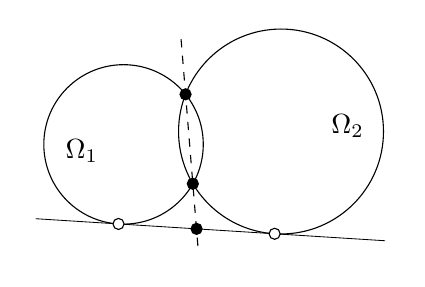
\begin{tikzpicture}[x=1.25cm,y=1.25cm]
			\clip (-1.3,-1.35) rectangle (2.45,1);
			\draw (-0.326,-0.186) circle (0.81);
			\draw (1.274,-0.055) circle (1.041);
			\coordinate (P) at (0.304,0.323);
			\coordinate (Q) at (0.378,-0.586);
			\coordinate (T1) at (-0.377,-0.994);
			\coordinate (T2) at (1.209,-1.094);
			\coordinate (M) at (0.416,-1.044);
			\draw [dashed,shorten <=-2em,shorten >=-2.5em] (P) to (Q);
			\draw [line width=0.3,shorten <=-3em,shorten >=-4em] (T1) to (T2);
			%\path (T1) to node[pos=0.55,sloped] {$\scriptscriptstyle |$} (M) to node[pos=0.45,sloped] {$\scriptscriptstyle |$} (T2);
			\draw[fill=black] (P) circle (2pt);
			\draw[fill=black] (Q) circle (2pt);
			\draw[fill=white] (T1) circle (2pt);
			\draw[fill=white] (T2) circle (2pt);
			\draw[fill=black] (M) circle (2pt);
			\node at (-0.75,-0.25) {$\Omega_1$};
			\node at (1.95,0) {$\Omega_2$};
		\end{tikzpicture} & & 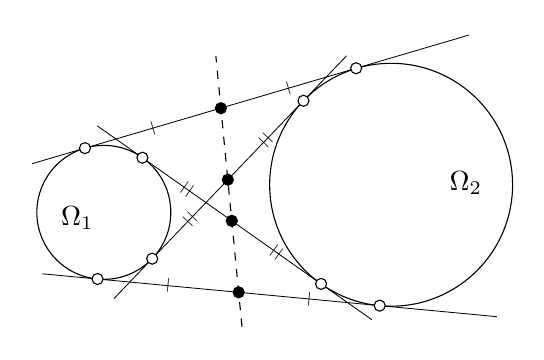
\begin{tikzpicture}[x=1.05cm,y=1.05cm]
			\clip (-2.25,-1.68) rectangle (3.65,2);
			\draw (-1.329,-0.234) circle (0.81);
			\draw (2.146,0.1) circle (1.469);
			\coordinate (S1) at (-1.405,-1.04);
			\coordinate (S2) at (2.008,-1.362);
			\coordinate (T1) at (-1.557,0.543);
			\coordinate (T2) at (1.723,1.509);
			\coordinate (U1) at (-0.744,-0.794);
			\coordinate (U2) at (1.086,1.116);
			\coordinate (V1) at (-0.862,0.427);
			\coordinate (V2) at (1.299,-1.099);
			\coordinate (K) at (0.302,-1.201);
			\coordinate (L) at (0.087,1.026);
			\coordinate (M) at (0.171,0.161);
			\coordinate (N) at (0.219,-0.336);
			\draw [dashed,shorten <=-1.25em,shorten >=-1.9em] (K) to (L);
			\draw [line width=0.3,shorten <=-2em,shorten >=-4.25em] (S1) to (S2);
			\draw [line width=0.3,shorten <=-2em,shorten >=-4.25em] (T1) to (T2);
			\draw [line width=0.3,shorten <=-2em,shorten >=-2.25em] (U1) to (U2);
			\draw [line width=0.3,shorten <=-2em,shorten >=-2.25em] (V1) to (V2);
			\path (S1) to node[sloped] {$\scriptscriptstyle |$} (K) to node[sloped] {$\scriptscriptstyle |$} (S2);
			\path (T1) to node[sloped] {$\scriptscriptstyle |$} (L) to node[sloped] {$\scriptscriptstyle |$} (T2);
			\path (U1) to node[sloped] {$\scriptscriptstyle ||$} (M) to node[sloped] {$\scriptscriptstyle ||$} (U2);
			\path (V1) to node[sloped] {$\scriptscriptstyle ||$} (N) to node[sloped] {$\scriptscriptstyle ||$} (V2);
			\draw[fill=black] (K) circle (2pt);
			\draw[fill=black] (L) circle (2pt);
			\draw[fill=black] (M) circle (2pt);
			\draw[fill=black] (N) circle (2pt);
			\draw[fill=white] (S1) circle (2pt);
			\draw[fill=white] (S2) circle (2pt);
			\draw[fill=white] (T1) circle (2pt);
			\draw[fill=white] (T2) circle (2pt);
			\draw[fill=white] (U1) circle (2pt);
			\draw[fill=white] (U2) circle (2pt);
			\draw[fill=white] (V1) circle (2pt);
			\draw[fill=white] (V2) circle (2pt);
			\node at (-1.65,-0.3) {$\Omega_1$};
			\node at (3.05,0.125) {$\Omega_2$};
		\end{tikzpicture} & \\\addlinespace
	\end{tabularx}
	Die Potenzgerade von $\Omega_1$~und~$\Omega_2$ in zwei Fällen.
\end{figure}
Potenzgeraden sind interessant, weil einige kanonisch auftretende Punkte auf ihnen liegen. Wenn sich $\Omega_1$~und~$\Omega_2$ zum Beispiel in zwei Punkten $P$~und~$Q$ schneiden, dann liegen $P$~und~$Q$ beide auf der Potenzgeraden von $\Omega_1$~und~$\Omega_2$, denn sie haben Potenz~$0$ bezüglich beider Kreise. In diesem Fall ist die Potenzgerade also einfach die Gerade~$PQ$. Sei ferner $t$ eine gemeinsame Tangente an $\Omega_1$~und~$\Omega_2$ mit Berührpunkten $T_1$,~$T_2$. Wenn sich $\Omega_1$ und $\Omega_2$ schneiden, kommen für $t$ nur die beiden äußeren gemeinsamen Tangenten in Frage. Wenn sich $\Omega_1$ und $\Omega_2$ hingegen nicht schneiden, können wir für $t$ auch die beiden inneren gemeinsamen Tangenten wählen. In jedem Fall liegt der Mittelpunkt von~$\overline{T_1T_2}$ auf der Potenzgeraden, was sofort aus der zweiten alternativen Beschreibung folgt.

Außerdem haben wir den folgenden, sehr nützlichen Fakt:
\begin{satzmitnamen}[Potenzzentrum dreier Kreise]
	Seien $\Omega_1$,~$\Omega_2$ und~$\Omega_3$ drei paarweise nicht-konzentrische Kreise. Sei $p_{1,2}$ die Potenzgerade von $\Omega_1$~und~$\Omega_2$ und definiere $p_{2,3}$,~$p_{3,1}$ analog.
	% Tien: Wie wäre es, wenn du auf die Kommas in den Subskripten verzichtest? Das sind schon viele Kommas in hintereinander. Ich habe mal \, eingefügt.
	Dann schneiden sich $p_{1,2}$,~$p_{2,3}$ und~$p_{3,1}$ in einem Punkt \embrace{oder sind paarweise parallel}.
	
	Insbesondere gilt: Wenn sich die Kreise $\Omega_1$,~$\Omega_2$ und~$\Omega_3$ paarweise schneiden, dann treffen sich die drei Verbindungsgeraden der Schnittpunkte in einem Punkt \embrace{oder sind paarweise parallel}.
\end{satzmitnamen}

\begin{figure}[ht]
	\centering
	\begin{tabularx}{\textwidth}{X c X c X}
		& 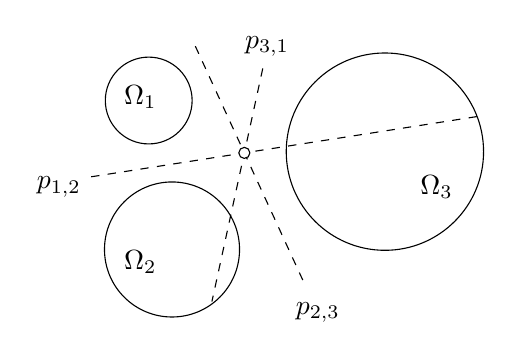
\begin{tikzpicture}[x=1.75cm,y=1.75cm]
			\draw (-2.139,0.675) circle (0.315);
			\draw (-1.97,-0.406) circle (0.49);
			\draw (-0.425,0.304) circle (0.716);
			\coordinate (K) at (-2.457,0.137);
			\coordinate (L) at (-1.021,-0.628);
			\coordinate (M) at (-1.397,0.515);
			\coordinate (Z) at (-1.445,0.295);
			\draw[dashed,shorten <=-0.5em,shorten >=-8.8em] (K) node[shift={(195:4ex)}] {$p_{1,2}$} to (Z);
			\draw[dashed,shorten <=-0em,shorten >=-4.5em] (L) node[shift={(295:3ex)}] {$p_{2,3}$} to (Z);
			\draw[dashed,shorten <=-2em,shorten >=-5.5em] (M)node[shift={(78:6.5ex)}] {$p_{3,1}$} to (Z);
			\draw[fill=white] (Z) circle (2pt);
			\node at (-2.2,0.7) {$\Omega_1$};
			\node at (-2.2,-0.5) {$\Omega_2$};
			\node at (-0.05,0.05) {$\Omega_3$};
		\end{tikzpicture} & & 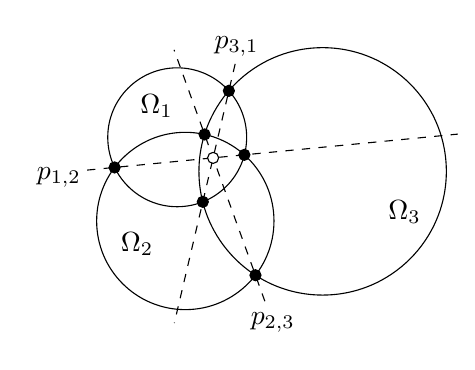
\begin{tikzpicture}
			\draw (-1.839,0.954) circle (0.882);
			\draw (-1.736,-0.109) circle (1.126);
			\draw (0.008,0.521) circle (1.571);
			\coordinate (S1) at (-2.634,0.571);
			\coordinate (S2) at (-0.986,0.731);
			\coordinate (T1) at (-1.514,0.134);
			\coordinate (T2) at (-1.183,1.544);
			\coordinate (U1) at (-1.491,0.99);
			\coordinate (U2) at (-0.845,-0.798);
			\coordinate (Z) at (-1.383,0.692);
			\draw[dashed,shorten <=-1em,shorten >=-7.75em] (S1) to (S2);
			\draw[dashed,shorten <=-1em,shorten >=-4.5em] (T2) to (T1);
			\draw[dashed,shorten <=-1em,shorten >=-3.25em] (U2) to (U1);
			\draw[fill=black] (S1) circle (2pt) node[shift=(190:4.75ex)] {$p_{1,2}$};
			\draw[fill=black] (S2) circle (2pt);
			\draw[fill=black] (T1) circle (2pt);
			\draw[fill=black] (T2) circle (2pt) node[shift=(80:3.75ex)] {$p_{3,1}$};
			\draw[fill=black] (U1) circle (2pt);
			\draw[fill=black] (U2) circle (2pt) node[shift=(290:4.25ex)] {$p_{2,3}$};
			\draw[fill=white] (Z) circle (2pt);
			\node at (-2.1,1.35) {$\Omega_1$};
			\node at (-2.35,-0.4) {$\Omega_2$};
			\node at (1.05,0) {$\Omega_3$};
		\end{tikzpicture} & \\\addlinespace
	\end{tabularx}
	Die paarweisen Potenzgeraden von $\Omega_1$,~$\Omega_2$ und~$\Omega_3$ in zwei Fällen.
\end{figure}

\begin{proof}
	Wenn die drei Potenzgeraden nicht paarweise parallel sind, dürfen wir ohne Beschränkung der Allgemeinheit annehmen, dass sich $p_{1,2}$~und~$p_{2,3}$ in einem Punkt~$Z$ schneiden. Dann hat $Z$ die gleiche Potenz bezüglich $\Omega_1$,~$\Omega_2$ und~$\Omega_3$. Also liegt $Z$ auch auf~$p_{2,3}$.
\end{proof}

Wir wollen nun Potenzgeraden benutzen, um einen Satz über Tangentensechsecke zu beweisen.

\begin{satzmitnamen}[Satz von Brianchon]
	Sei $ABCDEF$ ein konvexes Tangentensechseck. Dann schneiden sich die Hauptdiagonalen $AD$, $BE$ und~$CF$ in einem Punkt.
\end{satzmitnamen}

\begin{figure}[ht]
	\centering
	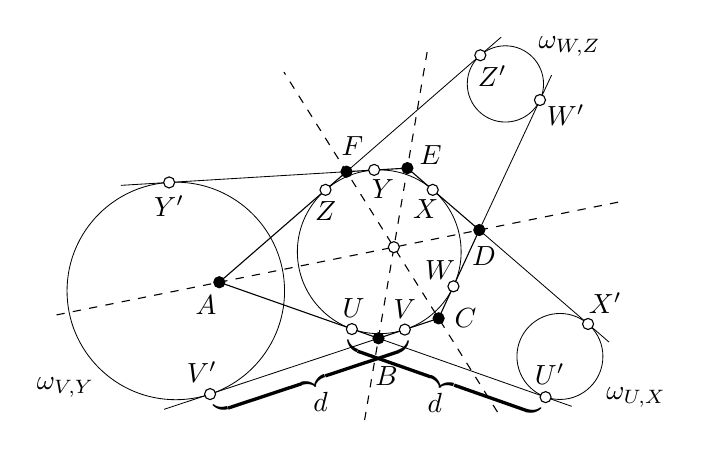
\begin{tikzpicture}[x=3.25cm,y=3.25cm]
		\draw [line width=0.3] (-1.529,-0.184) circle (0.425);
		\draw [line width=0.3] (-0.028,-0.44) circle (0.168);
		\draw [line width=0.3] (-0.241,0.625) circle (0.149);
		\draw [line width=0.3] (-0.734,-0.031) circle (0.32);
		\coordinate (A) at (-1.359,-0.15);
		\coordinate (B) at (-0.737,-0.369);
		\coordinate (C) at (-0.502,-0.291);
		\coordinate (D) at (-0.343,0.054);
		\coordinate (E) at (-0.624,0.296);
		\coordinate (F) at (-0.862,0.282);
		\coordinate (U) at (-0.841,-0.333);
		\coordinate (U1) at (-0.084,-0.599);
		\coordinate (V) at (-0.634,-0.335);
		\coordinate (V1) at (-1.395,-0.587);
		\coordinate (W) at (-0.444,-0.166);
		\coordinate (W1) at (-0.106,0.562);
		\coordinate (X) at (-0.525,0.211);
		\coordinate (X1) at (0.082,-0.313);
		\coordinate (Y) at (-0.754,0.289);
		\coordinate (Y1) at (-1.555,0.24);
		\coordinate (Z) at (-0.944,0.211);
		\coordinate (Z1) at (-0.339,0.737);
		\coordinate (P) at (-0.677,-0.013);
		\draw (A) to (B) to (C) to (D) to (E) to (F) to cycle;
		\draw[line width=0.3,shorten >=-1em] (B) to (U1);
		\draw[line width=0.3,shorten >=-1.75em] (B) to (V1);
		\draw[line width=0.3,shorten >=-1em] (D) to (W1);
		\draw[line width=0.3,shorten >=-1em] (D) to (X1);
		\draw[line width=0.3,shorten >=-1.75em] (F) to (Y1);
		\draw[line width=0.3,shorten >=-1em] (F) to (Z1);
		\draw [dashed,shorten <=-6em,shorten >=-5.25em] (A) to (D);
		\draw [dashed,shorten <=-3em,shorten >=-4.25em] (B) to (E);
		\draw [dashed,shorten <=-4em,shorten >=-4.25em] (C) to (F);
		\draw[fill=black] (A) circle (2pt) node[shift={(240:2.25ex)}] {$A$};
		\draw[fill=black] (B) circle (2pt) node[shift={(282:3.25ex)}] {$B$};
		\draw[fill=black] (C) circle (2pt) node[shift={(0:2.25ex)}] {$C$};
		\draw[fill=black] (D) circle (2pt) node[shift={(280:2.25ex)}] {$D$};
		\draw[fill=black] (E) circle (2pt) node[shift={(30:2.25ex)}] {$E$};
		\draw[fill=black] (F) circle (2pt) node[shift={(77:2.25ex)}] {$F$};
		\draw[fill=white] (U) circle (2pt) node[shift={(85:1.75ex)}] {$U$};
		\draw[fill=white] (V) circle (2pt) node[shift={(90:1.75ex)}] {$V$};
		\draw[fill=white] (W) circle (2pt) node[shift={(130:1.75ex)}] {$W$};
		\draw[fill=white] (X) circle (2pt) node[shift={(250:1.75ex)}] {$X$};
		\draw[fill=white] (Y) circle (2pt) node[shift={(295:1.75ex)}] {$Y$};
		\draw[fill=white] (Z) circle (2pt) node[shift={(270:1.75ex)}] {$Z$};
		\draw[fill=white] (U1) circle (2pt) node[shift={(80:2ex)}] {$U'$};
		\draw[fill=white] (V1) circle (2pt) node[shift={(110:2ex)}] {$V'$};
		\draw[fill=white] (W1) circle (2pt) node[shift={(-30:2.5ex)}] {$W'$};
		\draw[fill=white] (X1) circle (2pt) node[shift={(50:2.25ex)}] {$X'$};
		\draw[fill=white] (Y1) circle (2pt) node[shift={(270:2ex)}] {$Y'$};
		\draw[fill=white] (Z1) circle (2pt) node[shift={(300:2ex)}] {$Z'$};
		\draw[fill=white] (P) circle (2pt);
		\path
		(V) edge[draw=none] node[sloped,below=-0.01cm] {$\underbrace{\hspace{2.6cm}}$} node[sloped,shift={(270:3.5ex)}] (placeholder1) {} (V1)
		(U) edge[draw=none] node[sloped,below=-0.01cm] {$\underbrace{\hspace{2.6cm}}$} node[sloped,shift={(270:3.5ex)}] (placeholder2) {} (U1);
		\node at (placeholder1) {$d$};
		\node at (placeholder2) {$d$};
		\node at (0.27,-0.6) {$\omega_{U,X}$};
		\node at (-1.96,-0.56) {$\omega_{V,Y}$};
		\node at (0.01,0.77) {$\omega_{W,Z}$};
	\end{tikzpicture}
\end{figure}

\begin{proof}
	Wir wollen $AD$,~$BE$ und~$CF$ als Potenzgeraden von geeigneten Kreisen interpretieren. Dazu sei $\omega$ der Inkreis; die Berührpunkte mit den Seiten des Tangentensechsecks bezeichnen wir in dieser Reihenfolge mit $U$,~$V$, $W$, $X$, $Y$,~$Z$, sodass $U$~auf~$\overline{AB}$ liegt, $V$~auf~$\overline{BC}$ und so weiter. Wähle außerdem eine hinreichend große Länge $d>0$. Dann gibt es auf der Verlängerung von~$\overline{AB}$ über~$B$ hinaus einen Punkt~$U'$ mit $\abs{UU'}=d$ und auf der Verlängerung von~$\overline{BC}$ über~$B$ hinaus einen Punkt~$V'$ mit $\abs{VV'}=d$. Analog wählen wir Punkte $W'$~und~$X'$ auf den Verlängerungen von $\overline{CD}$ und~$\overline{DE}$ über~$D$ hinaus sowie $Y'$~und~$Z'$ auf den Verlängerungen von $\overline{EF}$ und~$\overline{FA}$ über~$F$ hinaus. Dann gibt es einen Kreis~$\omega_{U,X}$, der die Gerade~$AB$ in~$U'$ und die Gerade~$DE$ in~$X'$ berührt. Analog definieren wir Kreise $\omega_{V,Y}$ und~$\omega_{W,Z}$. Die Tangentenabschnitte $\overline{BU}$ und~$\overline{BV}$ sind gleich lang. Wegen $\abs{BU'}=d-\abs{BU}$ und $\abs{BV'}=d-\abs{BV}$ folgt, dass auch die Tangentenabschnitte $\overline{BU'}$ und~$\overline{BV'}$ gleich lang sind. Nach Eigenschaft~\ref{itm:PotenzTangente} liegt $B$ auf der Potenzgeraden der Kreise $\omega_{U,X}$~und~$\omega_{V,Y}$.
	% Tien: Vielleicht willst du Eigenschaft~2 referenzieren.
	Analoge Überlegungen lassen sich für die anderen Eckpunkte anstellen. Wir erhalten also in der Tat, dass $AD$,~$BE$ und~$CF$ die paarweisen Potenzgeraden der Kreise $\omega_{U,X}$,~$\omega_{V,Y}$ und~$\omega_{W,Z}$ sind. Somit schneiden sie sich in der Tat in einem Punkt (der parallele Fall kann nicht auftreten, da $ABCDEF$ konvex ist).
	% Tien: Konvexität hast du nicht vorausgesetzt.
\end{proof}

Der Satz von Brianchon ist nicht zuletzt dann nützlich, wenn er auf entartete Tangentensechsecke angewendet wird, in denen ein oder mehrere Eckpunkte auf dem Inkreis liegen (sodass die Innenwinkel an diesen Eckpunkten die Größe $180^\circ$ haben). Wir erhalten zum Beispiel folgenden bekannten Satz:

\begin{satzmitnamen}[Satz]
	Sei $ABCD$ ein Tangentenviereck und seien $W$,~$X$, $Y$ und~$Z$ die Berührpunkte des Inkreises mit den Seiten $\overline{AB}$, $\overline{BC}$, $\overline{CD}$ und~$\overline{DA}$. Dann schneiden sich die Diagonalen $AC$ und~$BD$ sowie die Geraden $WY$ und~$XZ$ in einem Punkt.
\end{satzmitnamen}

\begin{figure}[ht]
	\centering
	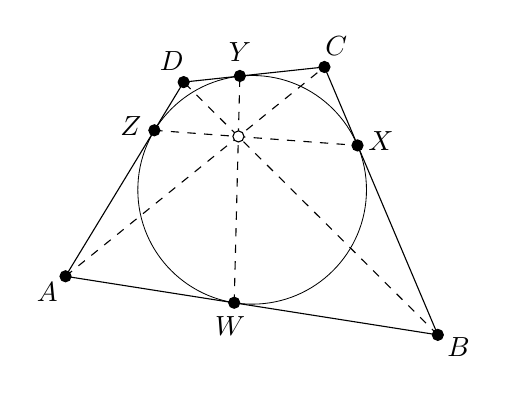
\begin{tikzpicture}[x=0.6cm,y=0.6cm]
		\draw [line width=0.3] (-0.26,-0.28) circle (2.42);
		\coordinate (A) at (-4.21,-2.11);
		\coordinate (B) at (3.67,-3.35);
		\coordinate (C) at (1.27,2.32);
		\coordinate (D) at (-1.71,2);
		\coordinate (W) at (-0.64,-2.67);
		\coordinate (X) at (1.97,0.66);
		\coordinate (Y) at (-0.52,2.13);
		\coordinate (Z) at (-2.33,0.98);
		\draw (A) to (B) to (C) to (D) to cycle;
		\draw [dashed] (W) to (Y);
		\draw [dashed] (Z) to (X);
		\draw [dashed] (A) to (C);
		\draw [dashed] (B) to (D);
		\draw [fill=black] (Y) circle (2pt) node[shift={(90:2ex)}] {$Y$};
		\draw [fill=black] (Z) circle (2pt) node[shift={(170:2ex)}] {$Z$};
		\draw [fill=black] (W) circle (2pt) node[shift={(260:2ex)}] {$W$};
		\draw [fill=black] (X) circle (2pt) node[shift={(10:2ex)}] {$X$};
		\draw [fill=black] (A) circle (2pt) node[shift={(220:2ex)}] {$A$};
		\draw [fill=black] (B) circle (2pt) node[shift={(330:2ex)}] {$B$};
		\draw [fill=black] (C) circle (2pt) node[shift={(60:2ex)}] {$C$};
		\draw [fill=black] (D) circle (2pt) node[shift={(120:2ex)}] {$D$};
		\draw [fill=white] (-0.55,0.85) circle (2pt);
	\end{tikzpicture}
\end{figure}

\begin{proof}
	Wende den Satz von Brianchon auf die entarteten Tangentensechsecke $AWBCYD$ und $ABXCDZ$ an.
\end{proof}

\subsection*{Beispielaufgaben}
Wie üblich findet ihr am Ende des Kapitels Tipps und am Ende des Heftes Lösungen zu den Beispielaufgaben.
\begin{aufgabe*}\label{aufgabe:VonAOPSGeklaut}
	Gegeben seien Kreise $\omega_1$~und~$\omega_2$, die sich in den Punkten $X$~und~$Y$ schneiden. Eine Gerade~$\ell_1$  durch den Mittelpunkt von~$\omega_1$ schneide~$\omega_2$ in den Punkten $P$~und~$Q$. Eine Gerade~$\ell_2$ durch den Mittelpunkt von~$\omega_2$ schneide~$\omega_1$ in den Punkten $R$~und~$S$. Zeige: Wenn $PQRS$ ein Sehnenviereck ist, dann liegt sein Umkreismittelpunkt auf der Gerade~$XY$.
\end{aufgabe*}

\begin{aufgabe*}\label{aufgabe:IMO1995_1}
	Die Punkte $A$,~$B$, $C$ und~$D$ liegen in dieser Reihenfolge auf einer Geraden~$\ell$. Der Kreis~$\omega_1$ mit Durchmesser~$\overline{AC}$ und der Kreis~$\omega_2$ mit Durchmesser~$\overline{BD}$ schneiden sich in den Punkten $X$~und~$Y$. Sei $Z$ der Schnittpunkt von~$XY$ mit der Strecke~$ \overline{BC}$ und sei $P$ ein innerer Punkt der Strecke~$\overline{XZ}$. Die Gerade~$CP$ schneide~$\omega_1$ außer in~$C$ noch in einem weiteren Punkt~$M$ und die Gerade~$BP$ schneide~$\omega_2$ außer in~$B$ noch in einem weiteren Punkt~$N$. Zeige, dass sich die Geraden $AM$, $DN$ und~$XY$ in einem Punkt schneiden.
\end{aufgabe*}

\begin{aufgabe*}\label{aufgabe:VAIMO2012_2}
	Das Dreieck $ABC$ sei bei~$C$ gleichschenklig. Sei $M$ ein innerer Punkt der Strecke~$\overline{BC}$. Auf der Verlängerung von~$\overline{AM}$ über~$M$ hinaus gebe es einen Punkt~$N$, für den $\abs{AN}=\abs{AC}$ gilt. Die Umkreise $\odot ABC$ und $\odot CMN$ schneiden sich außer in~$C$ noch in einem weiteren Punkt~$P$. Sei $Q$ der Schnittpunkt von $AB$~und~$CP$. Zeige, dass $Q$ auch auf der Winkelhalbierenden von $\winkel BMN$ liegt.
\end{aufgabe*}

\begin{aufgabe*}\label{aufgabe:Ceva+Brianchon}
	Sei $ABCD$ ein Tangentenviereck ist und seien $W$,~$X$, $Y$ und~$Z$ die Berührpunkte des Inkreises mit den Seiten $\overline{AB}$, $\overline{BC}$, $\overline{CD}$ und~$\overline{DA}$. Sei ferner $P$ der Schnittpunkt der Diagonalen $AC$ und~$BD$. Beweise
	\begin{equation*}
		\frac{\abs{AP}}{\abs{CP}}=\frac{\abs{AW}}{\abs{CX}}=\frac{\abs{AZ}}{\abs{CY}}\,.
	\end{equation*}
\end{aufgabe*}

\phantom{newpage}\vfill\hrule\vspace{-1em}

\subsection*{Tipps zu den Beispielaufgaben}

\textbf{Tipps zu Aufgabe~\ref{aufgabe:VonAOPSGeklaut}.} Betrachte die paarweisen Potenzgeraden der Kreise $\omega_1$, $\omega_2$ und $\odot PQRS$.

Wenn $O_1$, $O_2$ und $O$ die Mittelpunkte von $\omega_1$, $\omega_2$ und $\odot PQRS$ bezeichnen, dann betrachte den Höhenschnittpunkt des Dreiecks $OO_1O_2$.

\textbf{Tipp zu Aufgabe~\ref{aufgabe:IMO1995_1}.} Zeige, dass $BCNM$ und $ADNM$ Sehnenvierecke sind und benutze den Satz über das Potenzzentrum dreier Kreise.

\textbf{Tipps zu Aufgabe~\ref{aufgabe:VAIMO2012_2}.} Zeige, dass $AB$, $CP$ und die Winkelhalbierende von $\winkel BMN$ die paarweisen Potenzgeraden von $\odot ABC$, $\odot CMN$ und einem weiteren Kreis sind.

Welcher Kreis könnte dieser weitere Kreis sein? Mach dir eine genaue Skizze und stelle eine Vermutung auf. Beweise diese Vermutung dann mit einer Winkeljagd.

\textbf{Tipps zu Aufgabe~\ref{aufgabe:Ceva+Brianchon}.} Benutze den Satz von Ceva, um die Behauptung umzuformulieren.

Um die umformulierte Behauptung zu beweisen, kann zum Beispiel der Satz von Brianchon verwendet werden.